\documentclass{article}
\usepackage[tt=false]{libertine}
\usepackage{mathpartir}
\usepackage{amsthm}
\usepackage{graphicx}
\usepackage[colorlinks=true, citecolor=red]{hyperref}
\usepackage{bytefield}
\usepackage{listings}
\usepackage{microtype}
\usepackage{natbib}

\lstset{language=C}
\lstset{basicstyle=\ttfamily, columns=flexible}

\newcommand\Kwd[1]{{\sffamily\bfseries{#1}}}
\newcommand\EOf[4]{{#1}\vdash_{#2}{#3}:{#4}}
\newcommand\MOf[4]{{#1}\vdash_{#2}{#3}\div{#4}}
\newcommand\IsProc[3]{{#1}\vdash_{#2}{#3}\ \mathsf{proc}}
\newcommand\IsAction[3]{{#1}\vdash_{#2}{#3}\ \mathsf{action}}



\usepackage{sectsty}
\allsectionsfont{\sffamily}

\title{Implementing \Kwd{DNS} in \Kwd{C0}}
\author{Farzaneh Derakhshan \and Klaas Pruiksma \and Jonathan Sterling}

\newtheorem{theorem}{Theorem}[section]
\newtheorem{corollary}{Corollary}[theorem]
\newtheorem{lemma}[theorem]{Lemma}

\begin{document}

\maketitle

\begin{abstract}
  We have implemented a \Kwd{DNS} server in the \Kwd{C0} language, and
  evaluated it for both safety and performance.
\end{abstract}

\section{Background}


\Kwd{Domain Name System} (\Kwd{DNS}) is a hierarchical database that
maps domain names to IP addresses in a distributed manner augmented
with caching to achieve a better
performance~\citep{rfc:1034,rfc:1035,mun-lee:2005}. In fact, there are
three major parts:

\begin{enumerate}
\item Domain name space with resource records: The domain name space
  is a tree-like data structure with a root, and nodes labeled with at
  most 63 characters. The domain name of a label is the sequence of
  labels on the path from the node to the root. Each node of the tree,
  associated with a domain name, has a set of resource records.

\item Name servers keep information about a complete sub-tree of the
  domain name. They may also cache pointers to other name
  servers.

\item Resolvers are responsible for sending a query to name servers
  upon clients request and extract information from them. They may
  also have some parts of the name space cached themselves.  In fact,
  their role is to provide an interface between applications and DNS
  in the process of \emph{name resolution}. Name resolution starts
  when an application program (the host) sends its query for an IP
  address to a local name server, continues by the local name server
  which extracts the information in an iterative/recursive manner from
  different name servers (If it does not already have it in its own
  cache), and ends when the local name server returns the IP address
  to the host.
\end{enumerate}

The messages exchanged between host and name servers adhere to a
simple format, which is divided into 5 sections: (1) Header, (2)
Question, (3) Answer, (4) Authority, and (5) Additional.  Each of
these sections also has its own special format, some of which will be
covered in more detail in next parts of this document.


\subsection*{The \Kwd{C0} Language}\label{sec:c0}

The \Kwd{C0} programming language is a restricted subset of \Kwd{C}
that provides implicit memory safety to
programmers~\citep{pfenning:c0-reference}. Restrictions on pointer
arithmetic and casting, for example, allow the language to detect and
prevent any attempt to access an array out of its bounds. Furthermore,
there is no need for error-prone manual memory management, since
\Kwd{C0} is itself garbage-collected.

Further safety conditions can be enforced with contracts, which are a
class of assertions including loop invariants, pre- and
post-conditions, and dynamically checkable correctness conditions for
programs.

% \Kwd{Concurrent C0} (\Kwd{CC0}) is an extension of \Kwd{C0} that
% offers concurrency based on message passing by providing processes as
% the units of concurrent execution and channels as their message
% buffers~\citep{willsey-prabhu-pfenning:2016}. Concurrent processes
% communicate over channels using a protocol that is disciplined by
% session types~\citep{caires-pfenning-toninho:2013,
%   balzer-pfenning:2017}. In this protocol, each channel is typed such
% that it can either send or receive a message and, thus, it
% deliberately models the client/provider relation.

% However, the protocol is also able to characterize processes that are
% not completely sequential, and branch into different sequences as they
% encounter choices. This typing discipline also guarantees that data is
% sent and received in the correct order and by the correct processes
% (an invariant called \emph{session fidelity}), and that the
% communication is always one-to-one.



\section{Related Work}

\subsection*{Nail: parsing and generating data formats}

Marshalling and unmarshalling low-level data formats
is a highly error-prone process, requiring a great degree of care for
things like byte alignment, sign, etc.; mistakes in this kind of code
are responsible for numerous security vulnerabilities, especially when
written in unsafe languages like \Kwd{C}.

To ameliorate this difficulty, \citeauthor{bangert:2014} have
introduced \Kwd{Nail}, a specialized language for specifying low-level
data formats. \Kwd{Nail} specifications can then be compiled into real
parsers and formatters; as part of their evaluation, the authors of
\Kwd{Nail} have used it to develop a ``authoritative DNS server''.

\Kwd{Nail} has a number of interesting and extremely useful features,
including \emph{dependent fields}: these are used when the sort of
data in one field depends on the actual data of another field: for
instance, when a \verb|length| field is followed by an array of bytes
of that length.
%
Additionally, \Kwd{Nail} supports injecting user-supplied pairs of
partial inverses to wrap data in the generated parser and formatter;
this is crucial for compressed or encrypted data.

\paragraph{Evaluation}

We regard the \Kwd{Nail} project as an interesting point in the design
space, enabling rapid development of tools that interact with
low-level data formats. As far as safety is concerned, it is necessary
to trust two things:

\begin{enumerate}
\item The internal implementation of \Kwd{Nail}, which is written in
  \Kwd{C}. It is not clear to us what it means to trust \Kwd{C} code,
  because the ``semantics'' of \Kwd{C} code is completely informal and
  indefinite.
\item The user-provided implementations of any functions which are
  used for compression, decompression, etc. Indeed, there is reason to
  doubt the correctness of such code, even when written by experts;
  for instance, the \Kwd{DNS} demo in the \Kwd{Nail} development
  contains an operator precedence bug~\citep{nigeltao:ticket}.
\end{enumerate}

The issue described above suggests that while \Kwd{Nail} addresses
many difficulties, the most error-prone aspects of protocol
implementation are out of its scope. We think it would be an
interesting and worthwhile project to pursue a \emph{verified} version
of \Kwd{Nail} as a library for \Kwd{Coq}~\citep{coq:reference-manual},
enabling users to verify the correctness of their compression and
decompression functions relative to a formal approximation of
\Kwd{C}'s semantics.

Contrary to \Kwd{Nail}, our approach was to code parsers and
formatters for the \Kwd{DNS} data structures \emph{manually}, but in a
memory-safe and type-safe language. This means that while functional
correctness is not guaranteed, \emph{safety} is guaranteed.


\subsection*{The \Kwd{Fox} Project}
An earlier example of an implementation of the DNS protocol in a safe
and formally specified language is given by the \Kwd{Fox} project,
undertaken at Carnegie Mellon University in the
1990s~\citep{biagioni-harper-lee-milnes:1994,
  biagioni-harper-lee:2001}. Their principal artifact was a library
called \Kwd{FoxNet} which implemented an array of low-level network
infrastructure, including \Kwd{TCP}, \Kwd{IP}, \Kwd{ARP} and \Kwd{DNS}
in the \Kwd{Standard ML} language.

Unlike our development, \Kwd{FoxNet} had a highly modular character
which was enabled by the host language's sophisticated module system
(at the time, the only language to support signatures, structures and
generative functors, which are crucial for safe abstraction).


\subsection*{Other implementations}

More recently, safe languages
like \Kwd{Rust} and \Kwd{Go} have been gaining popularity. Both
languages have hosted implementations of the \Kwd{DNS}
protocol~\citep{github:trust-dns,github:miekg-dns}


\section{Our Project}\label{sec:our-project}

Our original project proposal was to develop a language for safe
concurrent programming with precise formal guarantees; however, the
negotiation process led us to choose a completely unrelated project,
which we describe in this section. We will be developing an
implementation of the DNS protocol in the memory-safe \Kwd{C0}
language (see \S\ref{sec:c0}); we have divided our work into two
principal components.

\subsection{Network interface}\label{sec:network-interface}

We have implemented a (limited) networking library for \Kwd{C0}. Due to limitations of the language, however, this library is not written entirely in \Kwd{C0} itself. Instead, we wrote a collection of small functions in \Kwd{C} which act as an interface between \Kwd{C0} code and the \Kwd{C} sockets library.

By splitting the library into these two parts, we can keep the \Kwd{C} portion of our codebase limited in scope. While our original plan was to never dynamically allocate memory in this code, we found that it was infeasible to use the socket functions without either dynamically allocating memory or violating other portions of our safety guarantees. As such, dynamically allocating memory was the safer choice, and so we have one allocation in each of the \texttt{sendto} and \texttt{recvfrom} functions. These are the only potentially unsafe regions of memory used in the application, and so we closely hand-checked their use for correctness. Additionally, we were able to ensure that any accesses to \Kwd{C0}-allocated memory are done so  using a collection of functions for safe memory access provided to libraries by the \Kwd{C0} runtime, ensuring safety of these accesses. As a result of this and the small size of the \Kwd{C} portion of the codebase, we can easily check all of the \Kwd{C} code for memory safety. Combining this with \Kwd{C0}'s memory safety, we ensure that any memory safety violations occur outside of our project (e.g. in the \Kwd{C} sockets library or in the OS).

Since this project is limited in scope to \Kwd{DNS}, we do not expose the full functionality of the sockets library in our network interface. We implemented functions that create and work with datagram-based sockets, as most of the network communication needed for \Kwd{DNS} is done via the datagram protocol \Kwd{UDP}. Additionally, to avoid busy-waiting, we provide a limited interface to the \texttt{poll} function of the \Kwd{C} standard library in much the same way. Finally, we add \Kwd{C0} interfaces for the collection of functions that translate between network and host byte order, in order to shift as much work as possible into \Kwd{C0}, rather than changing byte order in our \Kwd{C} code.

\subsection{Marshalling and unmarshalling}

Unlike \Kwd{C}, the \Kwd{C0} language has only a single type of
integers, which are represented internally as 32-bit integers. The
network interface (see \S\ref{sec:network-interface}) will deal with
requests and responses formatted as arrays of 32-bit integers; it is
the responsibility of the marshalling-and-unmarshalling module to
unpack this data into structured representations of core DNS
datatypes.

\begin{figure}
  \centering
  \begin{bytefield}[bitwidth=1.5em]{16}
    \wordbox{1}{\texttt{ID}}
    \\
    \bitbox{1}{\texttt{QR}}
    \bitbox{4}{\texttt{Opcode}}
    \bitbox{1}{\texttt{AA}}
    \bitbox{1}{\texttt{TC}}
    \bitbox{1}{\texttt{RD}}
    \bitbox{1}{\texttt{RA}}
    \bitbox{3}{\texttt{Z}}
    \bitbox{4}{\texttt{RCODE}}
    \\
    \wordbox{1}{\texttt{QDCOUNT}}
    \\
    \wordbox{1}{\texttt{ANCOUNT}}
    \\
    \wordbox{1}{\texttt{NSCOUNT}}
    \\
    \wordbox{1}{\texttt{ARCOUNT}}
  \end{bytefield}
  \caption{The layout specification of message headers in
    DNS.}\label{fig:layout-message-header}
\end{figure}


\begin{figure}
  \centering
  \begin{bytefield}{16}
    \wordbox[lrt]{1}{\texttt{NAME}}\\
    \skippedwords\\
    \wordbox[lrb]{1}{}\\
    \wordbox{1}{\texttt{TYPE}}\\
    \wordbox{1}{\texttt{CLASS}}\\
    \wordbox{2}{\texttt{TTL}}\\
    \wordbox[lrt]{1}{\texttt{RDATA}}\\
    \skippedwords\\
    \wordbox[lrb]{1}{}
  \end{bytefield}
  \caption{The bit layout specification of resource records in
    DNS.}\label{fig:layout-resource-record}
\end{figure}

\begin{figure}
  \begin{lstlisting}[frame=single]
struct header {
  int id;
  int qr;
  int opcode;
  int aa;
  int tc;
  int rd;
  int ra;
  int z;
  int rcode;
  int qdcount;
  int ancount;
  int nscount;
  int arcount;
};

typedef struct header* header;
  \end{lstlisting}

  \begin{lstlisting}[frame=single]
struct domain_name {
  string label;
  struct domain_name* next;
};

typedef struct domain_name* domain_name;

struct resource_record {
  domain_name name;
  int type;
  int class;
  int ttl;
  int rd_length;
  int[] rdata;
};

typedef struct resource_record* resource_record;
  \end{lstlisting}
  \caption{Example DNS data structures in our \Kwd{C0} implementation.}\label{fig:c0-data-structures}
\end{figure}

For instance, Figure~\ref{fig:layout-message-header} shows the
bit-level layout of DNS message headers, and
Figure~\ref{fig:layout-resource-record} shows the same for resource
records; Figure~\ref{fig:c0-data-structures} shows how we code these
structures in our \Kwd{C0} implementation. To convert between these
structured representations and the sequences of words which are used
at the boundaries of the network
interface~(\S\ref{sec:network-interface}), we implement functions of
the following kind:

\begin{lstlisting}
domain_name parse_domain_name(cursor cur, int[] data);
resource_record parse_resource_record(cursor cur, int[] data);
header parse_header(cursor cur, int[] data);
\end{lstlisting}

\paragraph{The cursor abstraction}
In order to enable a style of coding which is less error-prone than
manual cursor-passing, we implemented an abstract type of imperative
cursors, which can be advanced or retreated by a certain number of
bits. Then, our low-level bit arithmetic utilities can be used to read
(or write) a certain number of bits at a certain offset from (resp.\
to) our stream of words.

It is important for the modularity of our development that cursors
represent not indices into the 32-bit cells of the message, but rather
bit-indices; this is because specific parts of DNS data structures may
only be a few bits long, so their parsers cannot move the cursor
forward a full word's length.

A sample of our parsing code can be found in the supplementary
appendix to this proposal (\S\ref{appendix:decompression}).

\paragraph{The implemented fragment}

We have implemented marshalling and unmarshalling for a sizable
fragment of the \Kwd{DNS} protocol, omitting only some rare or
experimental resource record types. Our parser for domain names
supports compression as specified in~\cite{rfc:1035} (see
Appendix~\ref{appendix:decompression} for our domain name routine);
however, during formatting we do not attempt to re-compress domain
names. This would be necessary for a serious implementation.

\paragraph{Tests}

We have implemented several tests to ensure correct roundtrip behavior
of the marshalling and unmarshalling routines by hand-coding instances
of the \Kwd{DNS} message structure.

\section{Evaluation}

\subsection{Correctness and Safety}

By virtue of having written the majority of our \Kwd{DNS} server in
the memory- and type-safe \Kwd{C0} language, we enjoy certain safety
guarantees that are either impossible or intractable to achieve for
mainstream \Kwd{C}-based implementations. In return, we have sacrificed
some performance, but it is hard to tell how much of our performance
trade-off was due to garbage collection vs.\ the unoptimized character of
our implementation (but see Section~\ref{sec:performance}).

\paragraph{Contracts in \Kwd{C0}}

One feature of \Kwd{C0} that we have found completely invaluable is
its notion of \emph{contract}, which are a lightweight form of
assertion which wraps the input and output boundaries of
procedures. Consider for instance the following code from our
low-level bit manipulation library:

\begin{lstlisting}
int get_mask(int index, int size)
//@requires size < 32 && size >= 0;
//@requires index < 32 && index >= 0;
{
    return ((1 << size) - 1) << index;
}

int get_bits(int index, int size, int data)
//@requires size < 32 && size >= 0;
//@requires index < 32 && index >= 0;
{
    return (data & get_mask(index, size)) >> index;
}

int set_bits(int data, int index, int size, int value)
//@requires size < 32 && size >= 0;
//@requires index < 32 && index >= 0;
{
    return (data & ~(get_mask(index, size))) | (value << index);
}
\end{lstlisting}

Here, we used contracts to ensure that we would not suffer from bit
shift range errors. The code did not begin with these contracts, but
in the course of debugging, these contracts were introduced; in every
instance, introducing contracts (shifting blame closer and closer to
call-sites) enabled us to easily determine and liquidate bugs.

The \Kwd{C0} compiler can be instructed to check contracts dynamically
during execution, or to generate code which ignores them. This is
helpful, since it is important to have debuggable errors when
developing, but in production one may not wish to incur the cost of
dynamic contract checks. While dynamic execution of contract checks
is already very useful, we feel that more advanced techniques such as
abstract interpretation and its special case, symbolic execution,
would be even more useful.

\subsection{Performance}\label{sec:performance}

In order to evaluate the performance of our nameserver (\Kwd{c0ns}), we used \Kwd{resperf}, from the freely available set of DNS benchmarking tools provided by~\cite{github:dnsperf2}. Since our nameserver is recursive, rather than authoritative (that is, it relies on remote nameservers for the ground truth), \Kwd{resperf} was a more suitable performance tool than \Kwd{dnsperf}.

As we were unable to find any existing data sets with realistic loads for testing, we created a data set of approximately 700,000 entries of A queries (which appear to be the most common) by turning each word in the system dictionary into three URLs to query. We believe that this meets the criteria suggested for performance testing in that it has a good mixture of real and nonexistent domain names, and as we need to be able to read resource records other than A when receiving messages from the remote servers that we query. Ideally, we would like to use a more varied dataset that reflects real-world usage, but this appears to work well enough for performance testing. One other issue with our dataset is that all queries in it are unique. While this does not matter for our nameserver, as it does not cache, were we to add caching, we would like to use a dataset with repetitions in order to test the effect of caching on performance.

We began by testing with the default settings of \Kwd{resperf}, wherein the number of queries being sent per second increases linearly from 0 to 100,000 over the course of a minute. We found, however, that this did not yield useful results, as the throughput capacity of \Kwd{c0ns} is so low by comparison. After adjusting parameters to get useful data, we found that setting a maximum of 100 queries per second over the same time interval of 60 seconds was suitable. We then tested both the checked (safe) and unchecked (not safe) versions of \Kwd{c0ns} with these parameters. Interestingly, the difference between the performance of the checked version (shown in Figure~\ref{fig:checked-perf}) and the performance of the unchecked version (shown in Figure~\ref{fig:unchecked-perf}) was minimal, suggesting that contract-checking provides little to no overhead at these speeds (though it is likely that with higher base throughput, the difference would become more evident).

We also note that our latency remains low up until about 20 seconds into the test, at which point the number of queries per second is around 33. The latency graphs thus support the conclusion that we can maintain sustained loads of around 30 queries per second (as suggested as well by the throughput graph), but past that point, we appear to have saturated the server, as latency continues to increase up to 45 seconds (at which point \Kwd{resperf} considers queries to have failed).

Because of the low throughput of our system, we did not find it useful to test against commercial nameservers, relying instead on previous work such as \cite{fagin2017making}, which suggests that commercial nameservers can handle loads on the order of 20,000 to 80,000 queries per second. With such a large magnitude of difference, even if commercial nameservers perform substantially worse on our benchmark than on the benchmarks that others have used, we still have around 1,000-3,000 times less throughput.

\begin{figure}[h]
    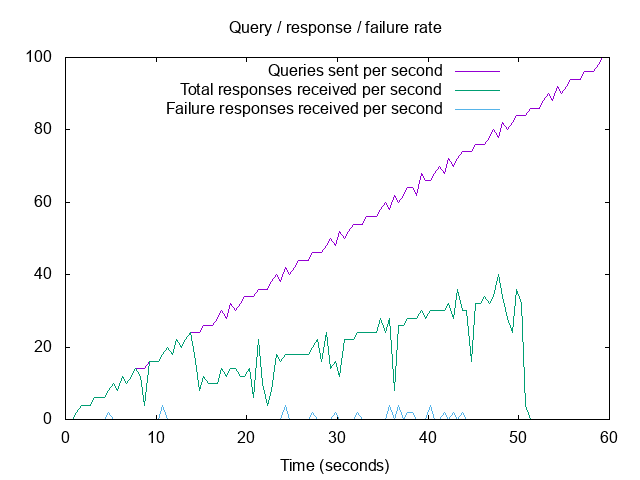
\includegraphics[width=0.5\textwidth]{unchecked_rate.png}
    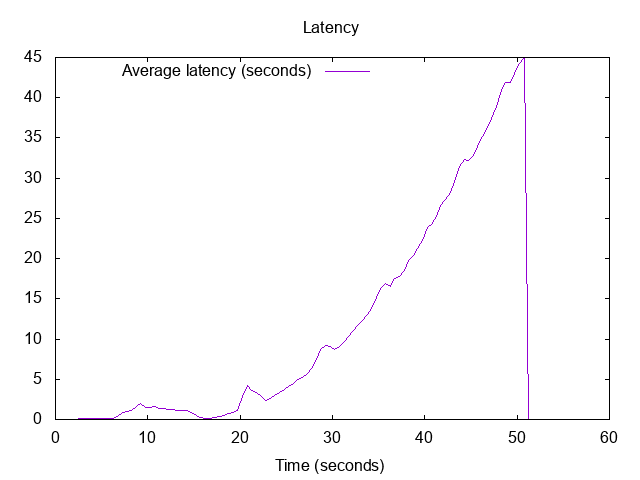
\includegraphics[width=0.5\textwidth]{unchecked_latency.png}
    \caption{Performance of the unchecked version of \Kwd{c0ns}}\label{fig:unchecked-perf}
\end{figure}

\begin{figure}[h]
    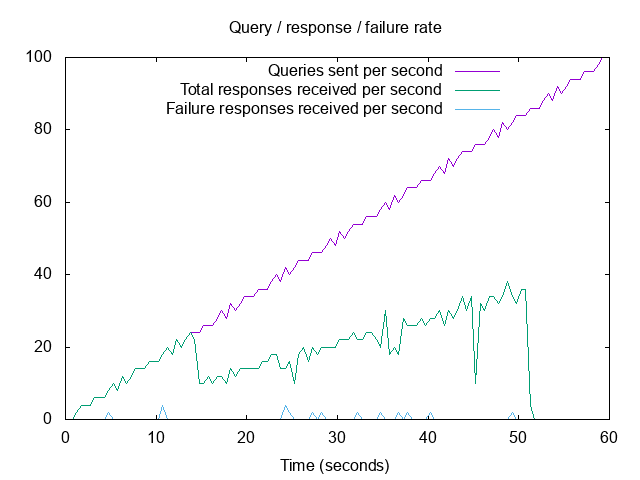
\includegraphics[width=0.5\textwidth]{checked_rate.png}
    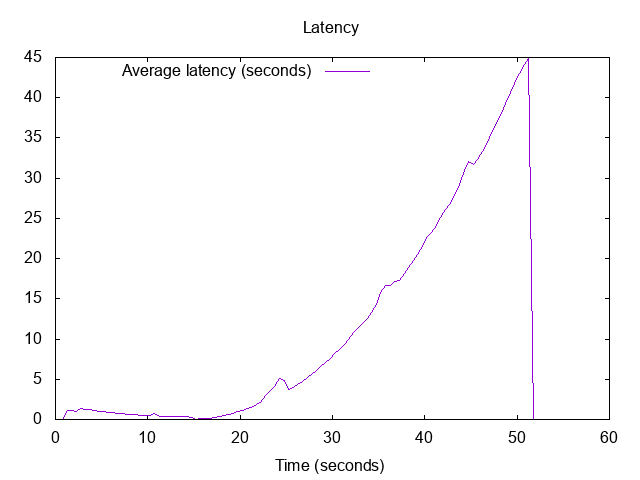
\includegraphics[width=0.5\textwidth]{checked_latency.png}
    \caption{Performance of the checked version of \Kwd{c0ns}}\label{fig:checked-perf}
\end{figure}

\section{Goals and Attainment}

We believe that this project meets our 75\% goal very solidly, but
falls short of the 100\% goal.\footnote{Our 75\% goal was to simply implement
  a working \Kwd{DNS} server; our 100\% goal was to extend this basic
  server with support for caching, and for further resource record
  types; we would also have liked to support compressing domain
  names. In our implementation, we supported only \emph{decompressing}
  domain names, which is allowed by the \Kwd{DNS} specification, but
  is not optimal~\citep{rfc:1035}.} The primary obstacle to finishing
the 100\% goal was that we underestimated the amount of time it would
take to clear up bugs relating to network byte order, which were the
source of much debugging time. While we believe that adding caching
would not be particularly difficult, given the structure of our
nameserver, there simply was not enough time to do so.

Moreover, from our testing, it appears that there are more pressing issues to fix with \Kwd{c0ns}. In  particular, our low performance even on benchmarks which do not benefit at all from caching suggests that perhaps we should focus on performance on unique queries before adding support for caching. In particular, we believe that performance could be greatly improved by adding support for concurrently processing requests, since resolving a query is network-bound (while we wait for the remote server to get back to us), and so should not block CPU-bound tasks like parsing other incoming queries.

% \section{Goals and Progress}

% \subsection*{75\%}

% Our 75\% goal is to develop a basic \Kwd{DNS} nameserver in \Kwd{C0}. In order to reduce the scope of this project, we restrict the types of resource data (and by extension, the types of queries) that we handle, and we will only provide support for \Kwd{UDP}-based queries. These two restrictions will simplify implementation, but leave enough functionality that we can evaluate our implementation both for correctness and for performance relative to other DNS implementations, as long as we restrict the test queries to those we have implemented.

% The bulk of this goal falls into the two components described in \S\ref{sec:our-project}, along with a small ``main'' component that uses these to actually handle queries. Currently, we have some unmarshalling functions and about a third of the network library implemented. We expect that the remainder of this goal should go fairly quickly --- marshalling is no harder than unmarshalling, and the network interface is relatively straightforward to implement once we have decided on what functions are necessary and what their arguments should be.

% \subsection*{100\%}

% To extend the above to a 100\% goal, we plan to extend the functionality of our nameserver by adding caching of requests and potentially adding to the types of resource data we support. While a nameserver without caching is not particularly useful, we believe that the portion of code most likely to contain memory errors is in some combination of reading data from the network and parsing that data --- in particular, dealing with message compression. As such, the 75\% goal is a proof of concept that demonstrates that these portions can be implemented safely, while the 100\% goal extends that proof of concept to be more useable (though still more limited than commercially available nameservers). We expect that in going from our 75\% version to the 100\% version, performance (and the scope of allowable queries) will increase and that we will be able to leave our arguments for correctness unchanged.

% \subsection*{125\%}

% We have two potential 125\% goals, depending on the outcome of our 100\% goal. If our nameserver has good performance relative to its competitors, we will work to provide better justification for the correctness of our nameserver, ideally arriving at a proof that statically verifies that all of our memory accesses are safe. In doing this, we will be able to safely turn off bounds checking when running our nameserver, increasing performance through verifying correctness. If instead our performance is very poor (or not helped much by turning off bounds checking), we will work to optimize our nameserver based on the results of performance testing. It is difficult to say what specifically we will do, but we plan to take the general approach of using software like \texttt{perf} to determine what portions of our code are bottlenecks, and trying to make those paths faster.

% \section{Evaluation Plan}

% Our evaluation breaks down into two parts --- one on the safety, and
% one on performance. As safety is a primary goal of this project, we
% plan to evaluate our code for safety. A large part of this will come
% for free from the memory safety guarantees of \Kwd{C0}, with the rest
% coming from a careful analysis of our \Kwd{C} code. This does have the
% disadvantage that \Kwd{C0}'s memory safety is checked dynamically,
% which incurs performance overhead. Ideally, as described in our 125\%
% goal, we would like to have a more static verification that memory
% safety holds, both to provide better performance, and as it provides
% better results than dynamic checking, since if a dynamic check fails,
% the program halts, which is less than ideal.

% For performance analysis, we plan to evaluate our nameserver for
% latency and throughput, as these appear to be the most important
% metrics for \Kwd{DNS} performance. We plan to do this using one of two
% pieces of software\citep{github:dnsperf1, github:dnsperf2}
% (confusingly, both named \texttt{dnsperf}), which read queries from a
% file and then send these requests to a nameserver. The tools mentioned
% in~\cite{github:dnsperf2} seem better-suited to our needs, as those
% of~\cite{github:dnsperf1} appear to not give latency information in a
% useful fashion.

% We will compare our results (at various load levels) to existing
% \Kwd{DNS} software (though we have yet to determine which specific
% software to take as our baseline). One remaining difficulty in
% evaluation lies in figuring out what sort of query workload to use ---
% the performance analysis tools we have looked at suggest using an
% input file with somewhere on the order of one million queries, which
% is more than can feasibly be generated by hand. However, there does
% not appear to be a standard benchmark for this testing as there are
% for many other systems. We will likely generate large test files in a
% randomized way, but do not have a good sense of how to make these
% files accurately reflect realistic usage.

\clearpage

\bibliographystyle{abbrvnat}
\bibliography{bibtex-references/refs,project}

\clearpage
\appendix
\section{Decompressing Domain Names}\label{appendix:decompression}

\begin{lstlisting}
domain_name parse_domain_name(cursor cur, int[] data)
//@requires cur != NULL;
//@requires cursor_get(cur) < \length(data) * 32;
//@requires cursor_get(cur) % 8 == 0;
{
    int orig_ix = cursor_get(cur);
    int len = read_bits(cur, data, 8);

    if (len == 0) {
        return domain_nil();
    }

    if ((len & 0xc0) == 0xc0) {
        // case: pointer
        // read the remaining bits of this word
        // as a pointer into the message (in octets)
        cursor_set(cur, orig_ix);
        int ptr = c0_ntohs(read_bits(cur, data, 16) & 0xFFFF);
        //@assert ((ptr & 0xc000) == 0xc000);
        ptr &= 0x3fff;

        cursor ptrCursor = cursor_new(ptr * 8);
        return parse_domain_name(ptrCursor, data);
    }

    // now we parse an ordinary label; we retreat by one octet
    // so that read_string can see the length cell
    cursor_retreat(cur, 8);
    string lbl = read_string(cur, data);
    return domain_cons(lbl, parse_domain_name(cur, data));
}
\end{lstlisting}

\end{document}
